\documentclass[tikz,border=8pt]{standalone}
\usepackage[T1]{fontenc}\usepackage{helvet}\renewcommand{\familydefault}{\sfdefault}
\usetikzlibrary{positioning,arrows.meta,fit,backgrounds}
\definecolor{naija}{HTML}{008751}
\definecolor{naijalight}{HTML}{ECFDF4}
\definecolor{ink}{HTML}{0F172A}
\definecolor{muted}{HTML}{64748B}
\begin{document}
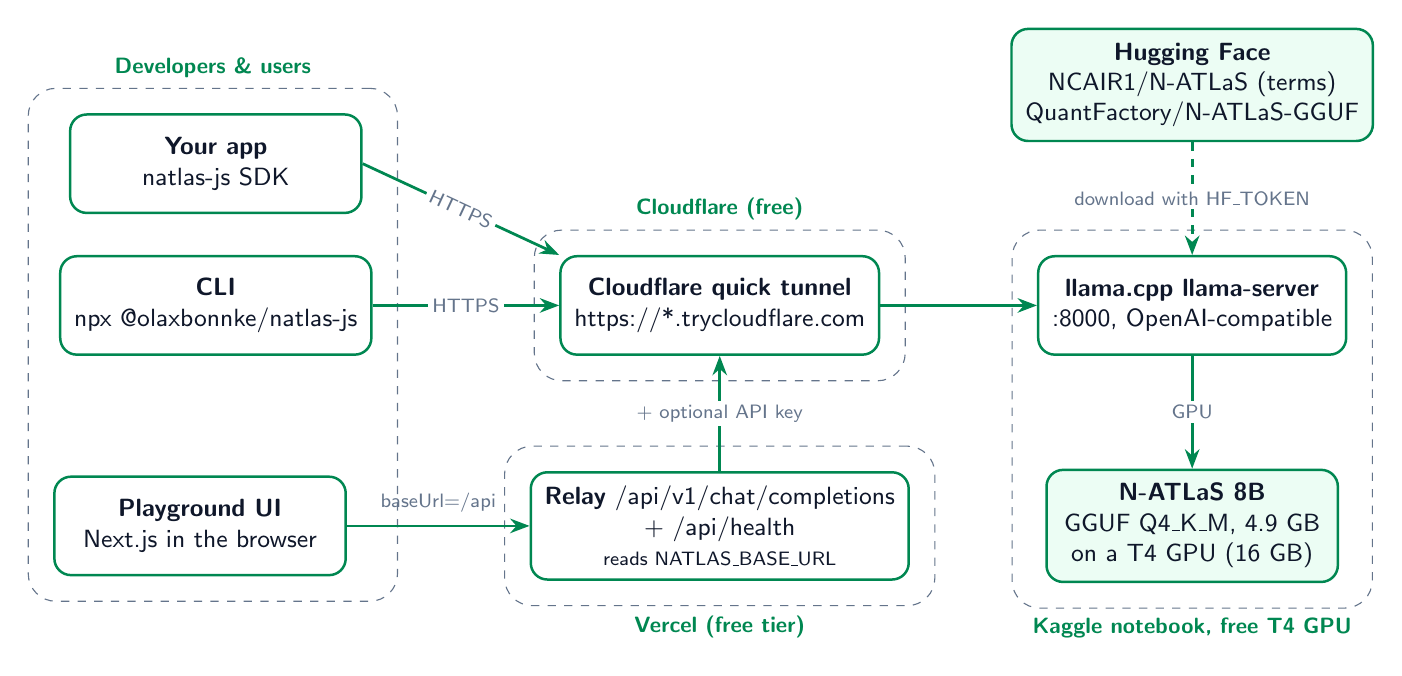
\begin{tikzpicture}[
  font=\small\color{ink},
  box/.style={draw=naija, line width=0.9pt, rounded corners=6pt, fill=white, align=center, minimum width=3.7cm, minimum height=1.25cm, inner sep=5pt},
  store/.style={box, fill=naijalight},
  group/.style={draw=muted, dashed, rounded corners=10pt, inner sep=9pt},
  lbl/.style={font=\footnotesize\bfseries\color{naija}},
  arr/.style={-{Stealth[length=7pt]}, line width=1pt, draw=naija},
  note/.style={font=\scriptsize\color{muted}, align=center, fill=white, inner sep=1.5pt},
]
\node[box] (sdk) at (0,3) {\textbf{Your app}\\ natlas-js SDK};
\node[box] (cli) at (0,1.2) {\textbf{CLI}\\ npx @olaxbonnke/natlas-js};
\node[box] (ui)  at (-0.2,-1.6) {\textbf{Playground UI}\\ Next.js in the browser};

\node[box] (tunnel) at (6.4,1.2) {\textbf{Cloudflare quick tunnel}\\ https://*.trycloudflare.com};
\node[box] (relay)  at (6.4,-1.6) {\textbf{Relay} /api/v1/chat/completions\\ + /api/health\\ \scriptsize reads NATLAS\_BASE\_URL};

\node[box] (server) at (12.4,1.2) {\textbf{llama.cpp llama-server}\\ :8000, OpenAI-compatible};
\node[store] (model) at (12.4,-1.6) {\textbf{N-ATLaS 8B}\\ GGUF Q4\_K\_M, 4.9 GB\\ on a T4 GPU (16 GB)};
\node[store] (hf) at (12.4,4.0) {\textbf{Hugging Face}\\ NCAIR1/N-ATLaS (terms)\\ QuantFactory/N-ATLaS-GGUF};

\begin{scope}[on background layer]
\node[group, fit=(sdk)(cli)(ui), label={[lbl]above:Developers \& users}] {};
\node[group, fit=(relay), label={[lbl]below:Vercel (free tier)}] {};
\node[group, fit=(tunnel), label={[lbl]above:Cloudflare (free)}] {};
\node[group, fit=(server)(model), label={[lbl]below:Kaggle notebook, free T4 GPU}] {};
\end{scope}

\draw[arr] (sdk.east) -- node[note, sloped]{HTTPS} (tunnel.north west);
\draw[arr] (cli.east) -- node[note]{HTTPS} (tunnel.west);
\draw[arr] (ui.east) -- node[note, above=3pt, fill=none]{baseUrl=/api} (relay.west);
\draw[arr] (relay.north) -- node[note]{+ optional API key} (tunnel.south);
\draw[arr] (tunnel.east) -- (server.west);
\draw[arr] (server.south) -- node[note]{GPU} (model.north);
\draw[arr, dashed] (hf.south) -- node[note]{download with HF\_TOKEN} (server.north);
\end{tikzpicture}
\end{document}
